Initial designs fitting to the project brief in \cref{Introduction Section} are formed based off of the current container models currently in use in \cref{Transport Containers for Nuclear Waste SubSection}. The current containers describe the importance of how the radioactive material in stored though the containers consume space and therefore are impractical in the long term where space consumption poses a serious problem as the United Kingdom plans to expand its nuclear power source.
\subsection{Design Ideas}
\label{Design Ideas SubSection}

The proposal is a container similar to that of the existing containers with space consumption in mind without sacrificing practicality, safety and effectiveness. The first problem to contend with is space consumption, many of the existing containers when stored or sent for disposal, waste space that could be used. The second problem is structural integrity during transportation and in storage, while a third concern is radiation exposure during the stages from extracting the radioactive materials from the nuclear power plants/ facilities to transport to unloading and processing to finally storage. \\ 

A hexagonal shape for the proposed container will allows for space saving either when the proposed design stand vertically or lies horizontally, geometry will allow the design to interlock. Though the design's size can be increased and decreased per specification of the radioactive waste load it will carry, two hexagonal barriers at either end to undergo the stress of the weight when the proposed design is stacked on top of each other. The two barriers will be larger than the interior hexagon in which the radioactive waste will be stored to allow for airflow for the built-up gases are able to leave the container.

\subsection*{Honeycomb Structure}
\label{Honeycomb Structure SubSection}

A honeycomb structure consists of a material laid out in combined hexagonal or octagonal pattern that is placed perpendicular to that of the surface area of another material shown in \cref{Honeycomb Image}, the benefit is the improved tensile strength to weight ratio of the material. A weak plastic formed into a honeycomb structure has the same strength to weight ratio as that of a sheet of weak metal, the aim is to use a light and weak material and improve its strength by not altering the material by making it into a composite or an alloy but by changing how the material handles a weight/ impact that is now dispersed of a wide area instead of a localised impact causing the material to weaken and ultimately fail. \\

The advantages of the honeycomb structure is that a design can be given the tensile strength of a solid block of metal with only a fraction of the weight. The use of a honeycomb structure in this theoretical design is useful as to pair it to lead, steel, aluminium and iron, some of which are heavy materials that can replace the effect of strength and lower the weight of the container, improving handling of the container. 

\subsection*{Carbon Nanotubes}
\label{Nano Tubes SubSection}

Carbon nanotube utilise the same hexagonal shape that the honeycomb structure does however the diameter of each individual strand is in nanometers. Carbon nanotube are woven onto a material where the much like the honeycomb structure improves the tensile strength of the original material, they have high thermal and electrical conductivity and hold a low thermal expansion co-efficient. However the carbon nanotubing is highly expensive to produce as a continuous laser cuts away at a graphite sheet to from the structure when cooled. Another way is where two carbon rods are place end to end as an electtode where a direct under is placed upon the two rods and the soot that is expelled contains the carbon nanotubes \cite{CarbonNano}. The carbon nanotube is beneficial not only to the proposed design but as an improvement to current containers as multiple carbon nanotube sheets can be placed on the surface of a material and increase its thermal conductivity and tensile strength. A disadvantage though is that its expensive to produce and therefore counter intuitive as future container must be affordable as increase in radioactive waste creates high demand for such containers.

\begin{figure}[H]
\centering
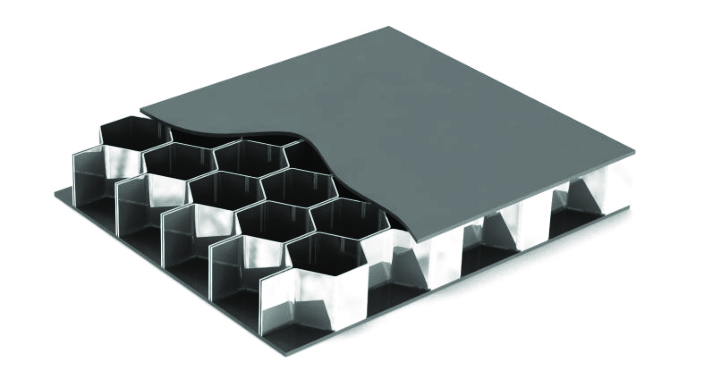
\includegraphics[scale=0.6]{Media/MaterialsResearch/Honeycomb-structure-Honeycomb-structures-are-highly-laborious-in-manufacturing-and.png}
\caption{Visual aid of the implementation of a honeycomb structure \cite{HoneycombPic}.}
\label{Honeycomb Image}
\end{figure}

\begin{figure}[H]
\centering
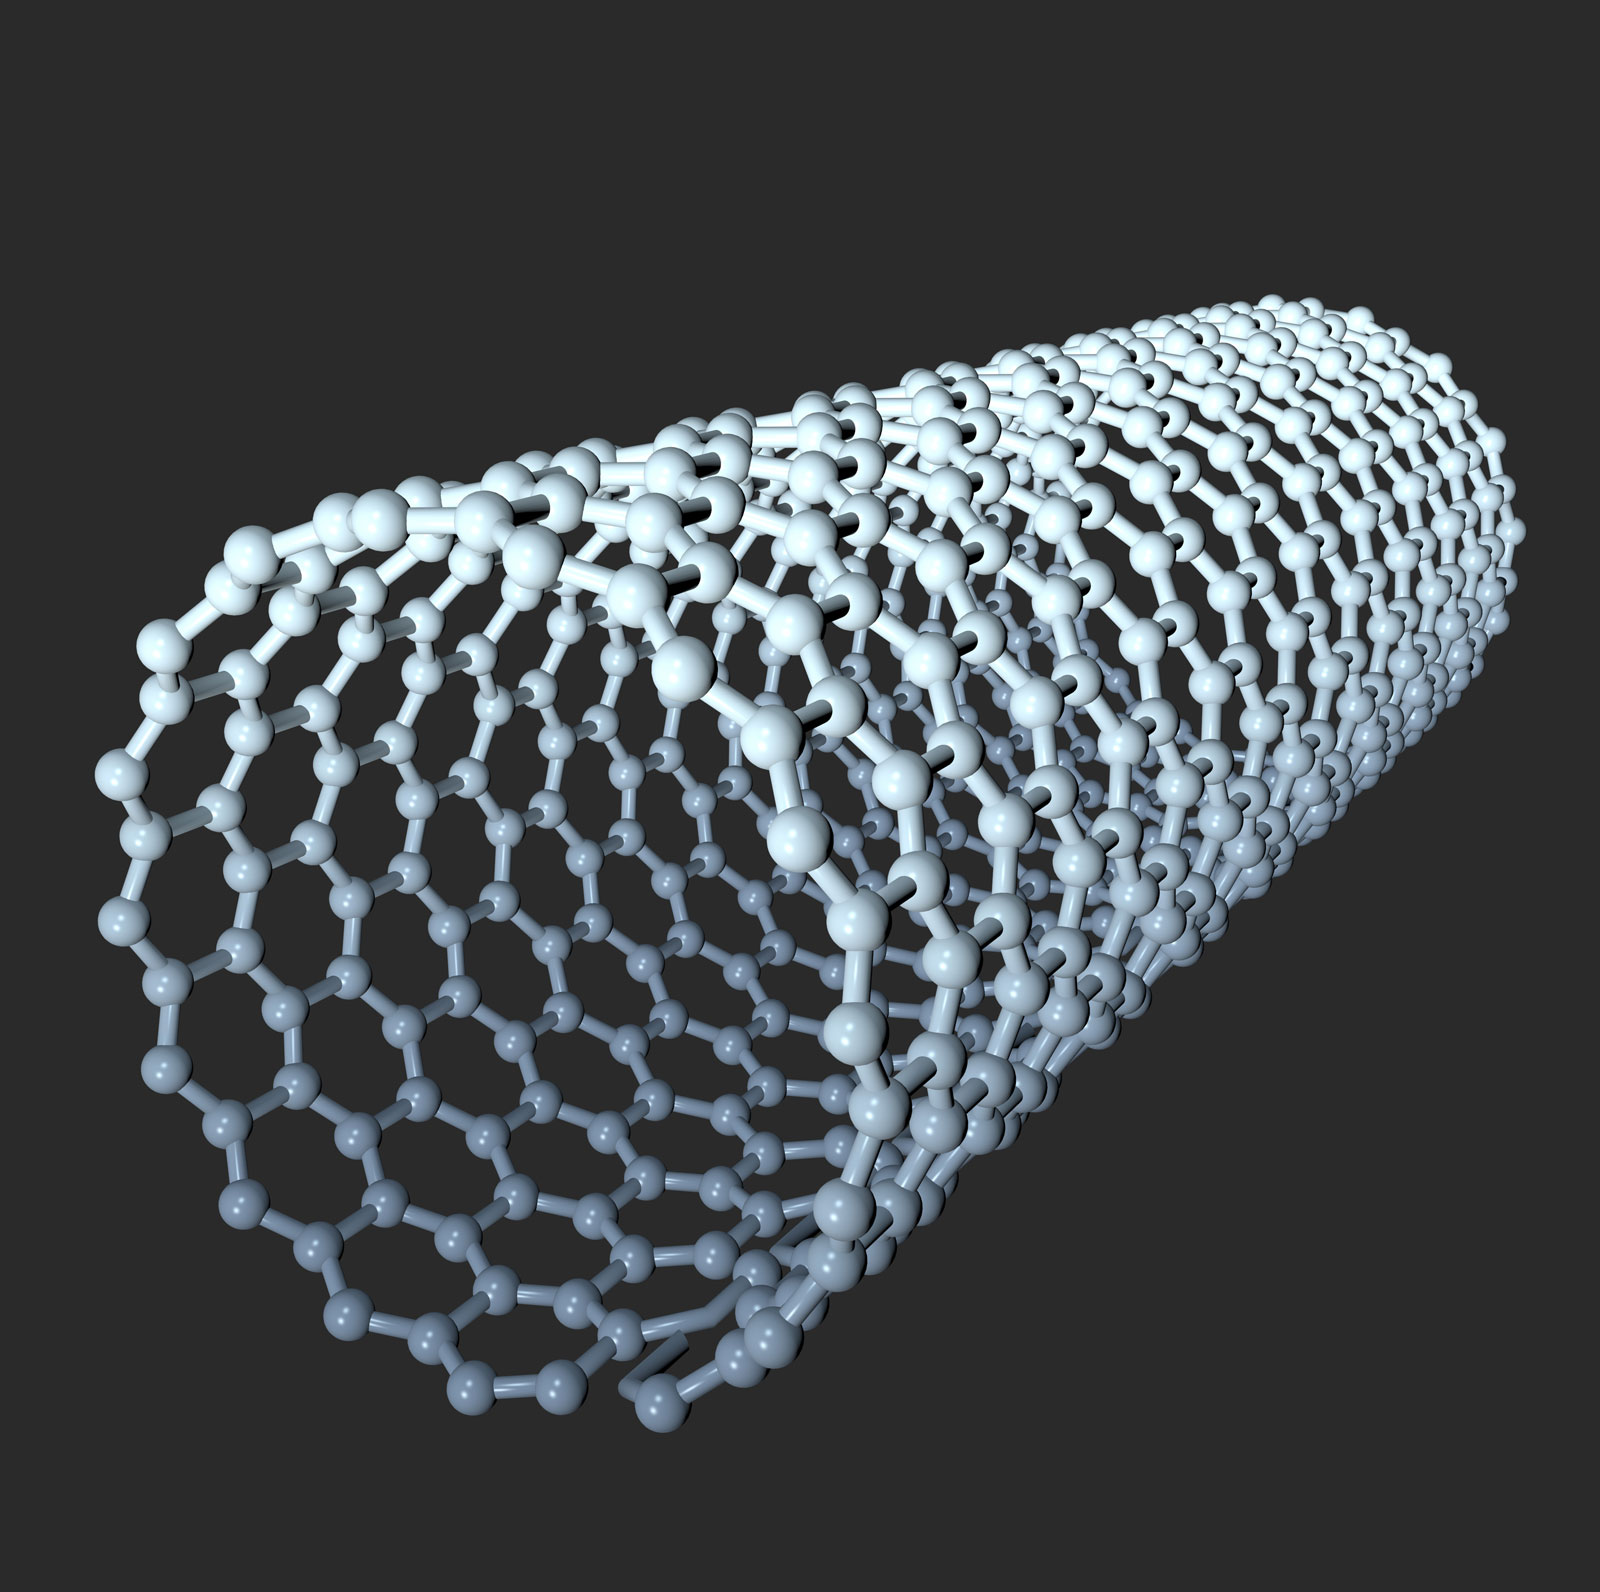
\includegraphics[scale=0.2]{Media/ProductDesign/Illustration-carbon-nanotube.jpg}
\caption{Illustration of a sheet of carbon nanotube \cite{CarbonNano}.}
\label{Carbon Nanotube image}
\end{figure}

\subsection{Proposed Design}
\label{Proposed Design SubSection}

The proposed design is addition to that of current containers for radioactive materials that is formed off the basis of the 500L drum in \cref{500 Litre Drum SubSubSection} and the Tru-Shield container in \cref{Tru-Shield Cylinder SubSubSection}. The use for the proposed design is that of instance storage where instead of the radioactive material being collected from the nuclear reactor facilities it's placed directly into the proposed design and then transported via rail or road to is treatment, storage and or disposal facility. The design for this type of transport limits the human interaction with the material as when the proposed design reaches the site its either filled with cement much like the 500L drum or put straight into storage. The proposed design can have the ability to be adapted to adopted lead plating to improve its radiation penetration resistance as proved in \cref{Data Analysis Section} where it shows as lead is such a dense material it blocks most of the gamma radiation that tries to pass through it. \\

The proposed design shown in \cref{Proposed Design} can have multiple openings whether it be vertical from the top where the lid can be screwed on and bolted in place much like the 500L drum or Tru-Shield. Another opening is horizontally where each side plate can be taken of similar to that of the lids and seals on concrete and steel boxes, where they are sealed on for long term storage. The orientation of the proposed design is how its to be stored and as each side plate can be taken off, the honeycomb structure as seen in \cref{Hexangonal Plate} can be filled with cement to further enforce the radioactivity resistance. Each side plate is connected to a steel strut running along the length of the proposed design as seen in \cref{Birds eye image} to improve the tensile strength, its further allows for the honeycomb structure to be 100\% effective. Sheet steel or aluminum is used as the external coat of the design as its malleable properties absorb the impact vibrations so not to damage to honeycomb structure that protects the integrity of the inner chamber that holds the radioactive material. \\

When ready for storage the proposed design can be stacked on top of one another whether it be horizontally or vertically shown in \cref{Circle and Hex Images}. The current 500L drum are of circular design that can only be placed vertically due to the lid and vent placement on top of the container whereas the proposed design can can the opening placed at multiple points depending on specifications meaning it can be stacked vertically or horizontally. The inner hexagon in smaller than the two outer barriers promotes airflow no matter how the proposed design's are stacked on top on one another or side by side, this allows for more containers to be stored and less space to be wasted. \\

Inside the inner hexagon will fit a stainless steel cylinder than can be externally lined with lead where to improve radioactivity resistance, the steel cylinder will hold the radioactive material where with a lead coating, no or little cement is needed to lower the radioactivity of the waste, if no lead exterior the cylinder can be access either from the top or a side panel to which then it's ready for storage. Upon regular checks on container health and radiation checks, the side panels protect the container from surface contact: scratches, corrosion and water where the honeycomb structure and carbon nanotubes project the container from high strength external contact: rocks falling, other container hitting it and being dropped by a crane. What ever hazard the container faces, the externally skin can be removed and reprocessed and the physically dimension of the proposed design does not change where with current models, they are placed into larger containers with pose a future physical space issue.

\newpage
\begin{multicols}{2}
\begin{figure}[H]
\centering
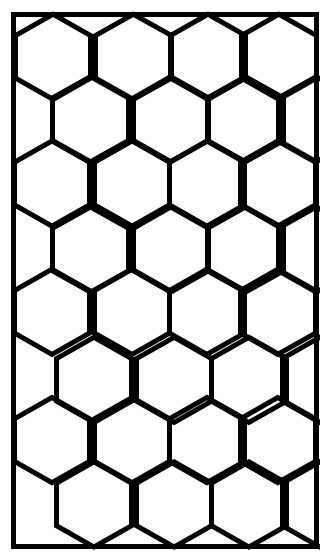
\includegraphics[scale=0.5]{Media/ProductDesign/HexPlate.png}
\caption{Layout of the side panel on the proposed design using a honeycomb structure.}
\label{Hexangonal Plate}
\end{figure}

\begin{figure}[H]
\centering
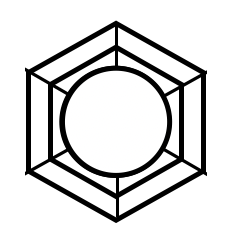
\includegraphics[scale=1.0]{Media/ProductDesign/BirdsEye.png}
\caption{A birds eye view of the proposed idea when placed vertically, showing all 6 side plates and the 6 support bars connecting each side plate.}
\label{Birds eye image}
\end{figure}
\end{multicols}

\begin{figure}[H]
\centering
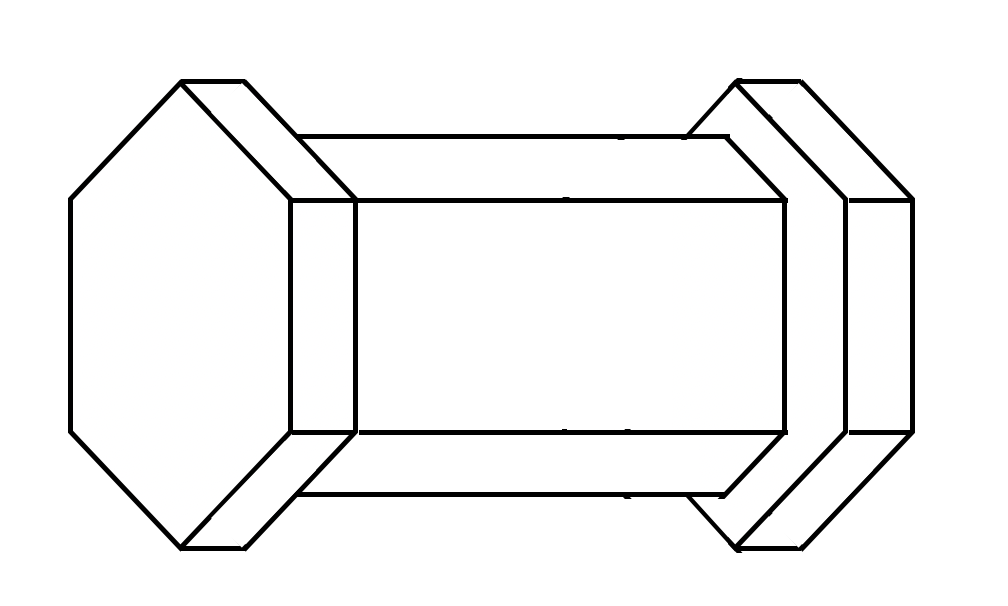
\includegraphics[scale=0.7]{Media/ProductDesign/Proposed Design.png}
\caption{Proposed design shape and outline, can either be placed horizontally or vertically.}
\label{Proposed Design}
\end{figure}

\begin{figure}[H]
\centering
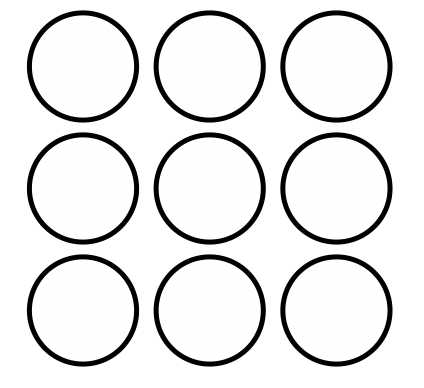
\includegraphics[scale=0.7]{Media/ProductDesign/Circle.png}
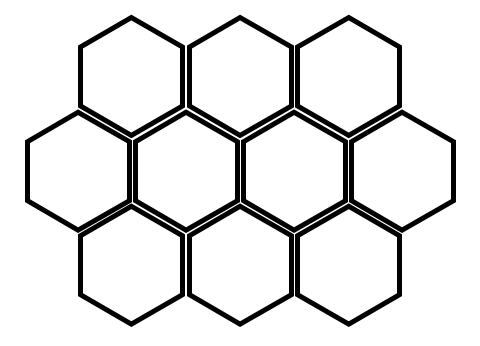
\includegraphics[scale=0.8]{Media/ProductDesign/Hex.png}
\caption{View of the current circular storage containers (Left) and of the storage of the proposed design (right) in either vertical or horizontal storage.}
\label{Circle and Hex Images}
\end{figure}

\subsection{Relative Merits of the Proposed Design}
\label{Relative Merits of the Proposed Design SubSection}

\subsubsection*{Proposed Design Advantages}
\label{Proposed Design Advantages SubSubSection}

The proposed design can be stacked on top of one another or alongside each other as depicting in \cref{Circle and Hex Images}, this saves space without restricting airflow due to the smaller hexagonal shape in the middle of the proposed design shown is \cref{Proposed Design}.\\

The radioactive materials can be place directly into the container at the nuclear reactor facility eliminating risk to human life. The proposed design isn't one fixed design, its customize straight from the factory in prediction for its plan in the future. \\

Furthermore the proposed design doesn't have to be placed in larger container to preserve the radioactive materials integrity whereas in the proposed design, new layers of sheet steel and aluminium can be applied thus maintaining the same sized container through tout its lifetime and only the exterior is affected. \\

As each side panel and the external metal surface is replaceable, it has the ability to use recycled materials and reused and re purpose old materials, thus this container has some sustainability.

\subsubsection*{Proposed Design Disadvantages}
\label{Proposed Design Disadvantages SubSubSection}

The proposed design is more complex than current containers that are centred around one single shape with minimal layers, making current designs easier to produce.Due to the ability to stack them, if corrosion in detect on a container at the bottom, all containers above need to be removed creating risk to human life. \\

If the proposed design is single use where the radioactive materials go into the design at the nuclear power facilites, the large proposed design much undergo transportation to the storage and disposal facility but 500L drum dues to the small size can be transported in greater quanitity.